% !TeX root = mos-en.tex

%%%%%%%%%%%%%%%%%%%%%%%%%%%%%%%%%%%%%%%%%%%%%%%%%%%%%%%%%%%%%%%%

\begin{prob}{Should you sample with or without replacement?\annotate{D}}
Urn $A$ contains $2$ red balls and $1$ green ball, and urn $B$ contains $101$ red balls and $100$ green balls. An urn is chosen at random and two balls are randomly drawn from the selected urn. You win if you correctly identify whether the selected urn was $A$ or $B$ based on the colors of the balls that were drawn.

Compute the probabilities of winning for each of the following rules and decide which gives you the highest probability of winning.

\que{1} The first ball is replaced before the second drawing.

\que{2} The first ball is not replaced before the second drawing.

\que{3} After the first ball is drawn you can decide whether it will be replaced or not.

\textbf{Hint:} When computing probabilities:
\[
\disfrac{101}{201}\approx \disfrac{100}{201} \approx \disfrac{100}{200} \approx \disfrac{1}{2}\,.
\]
\end{prob}

\solution{}

There are four outcomes which we denote by $RR, RG, GR, GG$. For each rule compute the conditional probabilities of the four outcomes given that urn $A$ or urn $B$ was selected initially. These probabilities must be multiplied by $1/2$ because the selection of an urn is random.

\ans{1} Drawing with replacement:
\[
\renewcommand*{\arraystretch}{1.5}
\begin{array}{lcccc}
P(RR|A) &=& \frac{2}{3} \cdot \frac{2}{3} &=& \frac{4}{9}\\
P(RR|B) &=& \frac{1}{2} \cdot \frac{1}{2} &=& \frac{1}{4}\\
\hline
P(RG|A) &=& \frac{2}{3} \cdot \frac{1}{3} &=& \frac{2}{9}\\
P(RG|B) &=& \frac{1}{2} \cdot \frac{1}{2} &=& \frac{1}{4}\\
\hline
P(GR|A) &=& \frac{1}{3} \cdot \frac{2}{3} &=& \frac{2}{9}\\
P(GR|B) &=& \frac{1}{2} \cdot \frac{1}{2} &=& \frac{1}{4}\\
\hline
P(GG|A) &=& \frac{1}{3} \cdot \frac{1}{3} &=& \frac{1}{9}\\
P(GG|B) &=& \frac{1}{2} \cdot \frac{1}{2} &=& \frac{1}{4}\end{array}
\]
If the outcome is $RR$ there is a higher probability that urn $A$ was selected ($4/9$) than that urn $B$ was selected ($1/4$); otherwise, there is a higher probability that urn $B$ was selected:
\[
P(\textsf{winning})=\frac{1}{2}\left(\frac{4}{9} + \frac{1}{4}+ \frac{1}{4}+ \frac{1}{4}\right)=\disfrac{43}{72}\approx 0.5972\,.
\]

\ans{2} Drawing without replacement:
\[
\renewcommand*{\arraystretch}{1.5}
\begin{array}{lcccc}
P(RR|A) &=& \frac{2}{3} \cdot \frac{1}{2} &=& \frac{1}{3}\\
P(RR|B) &=& \frac{1}{2} \cdot \frac{1}{2} &=& \frac{1}{4}\\
\hline
P(RG|A) &=& \frac{2}{3} \cdot \frac{1}{2} &=& \frac{1}{3}\\
P(RG|B) &=& \frac{1}{2} \cdot \frac{1}{2} &=& \frac{1}{4}\\
\hline
P(GR|A) &=& \frac{1}{3} \cdot 1 &=& \frac{1}{3}\\
P(GR|B) &=& \frac{1}{2} \cdot \frac{1}{2} &=& \frac{1}{4}\\
\hline
P(GG|A) &=& \frac{1}{3} \cdot 0 &=& 0\\
P(GG|B) &=& \frac{1}{2} \cdot \frac{1}{2} &=& \frac{1}{4}
\end{array}
\]
If the outcome is $GG$ there is (of course!) a higher probability that urn $B$ was selected than that urn $A$ was selected; otherwise, there is a higher probability that urn $A$ was selected:
\[
P(\textsf{winning})=\frac{1}{2}\left(\frac{1}{3} + \frac{1}{3}+ \frac{1}{3}+ \frac{1}{4}\right)=\frac{5}{8}=0.6250\,,
\]
which is greater than the probability of winning when sampling with replacement.

\ans{3} The decision is based on the outcome of the first draw.

If the first drawing is from urn $A$ the probabilities must also be conditioned on the decision to sample with or without replacement. Drawing first from urn $B$ does not affect the probabilities because of the approximation in the hint.
\[
\renewcommand*{\arraystretch}{1.5}
\begin{array}{lcccc}
P(RR|A,w) &=& \frac{2}{3} \cdot \frac{2}{3} &=& \frac{4}{9}\\
P(RR|A,w/o) &=& \frac{2}{3} \cdot \frac{1}{2} &=& \frac{1}{3}\\
P(RR|B) &=& \frac{1}{2} \cdot \frac{1}{2} &=& \frac{1}{4}\\
\hline
P(RG|A,w) &=& \frac{2}{3} \cdot \frac{1}{3} &=& \frac{2}{9}\\
P(RG|A,w/o) &=& \frac{2}{3} \cdot \frac{1}{2} &=& \frac{1}{3}\\
P(RG|B) &=& \frac{1}{2} \cdot \frac{1}{2} &=& \frac{1}{4}\\
\hline
%\end{array}
%\]
%\[
%\renewcommand*{\arraystretch}{1.5}
%\begin{array}{lcccc}
P(GR|A,w) &=& \frac{1}{3} \cdot \frac{2}{3} &=& \frac{2}{9}\\
P(GR|A,w/o) &=& \frac{1}{3} \cdot 1 &=& \frac{1}{3}\\
P(GR|B) &=& \frac{1}{2} \cdot \frac{1}{2} &=& \frac{1}{4}\\
\hline
P(GG|A,w) &=& \frac{1}{3} \cdot \frac{1}{3} &=& \frac{1}{9}\\
P(GG|A,w/o) &=& \frac{1}{3} \cdot 0 &=&0\\
P(GG|B) &=& \frac{1}{2} \cdot \frac{1}{2} &=& \frac{1}{4}\\\end{array}
\]
If a red ball is drawn first then $\frac{4}{9}>\frac{1}{4}$ and $\frac{2}{9}<\frac{1}{4}$ with replacement, whereas $\frac{1}{3}>\frac{1}{4}$ and $\frac{1}{3}>\frac{1}{4}$ without replacement, so the second ball can help identify the urn only if the drawing is done \emph{with} replacement: urn $A$ if red, urn $B$ if green. Choose draw with replacement:
\[
P(\textsf{winning if red first})=\frac{1}{2}\left(\frac{4}{9}+\frac{1}{4}\right)=\frac{25}{72}\,.
\]
If a green ball is drawn first then $\frac{2}{9}<\frac{1}{4}$ and $\frac{1}{9}<\frac{1}{4}$ with replacement, whereas $\frac{1}{3}>\frac{1}{4}$ and $0<\frac{1}{4}$ without replacement, so the second ball can help identify the urn only if the drawing is done \emph{without} replacement: urn $A$ if red, urn $B$ if green. Choose draw without replacement:
\[
P(\textsf{winning if green first})=\frac{1}{2}\left(\frac{1}{3}+\frac{1}{4}\right)=\frac{7}{24}\,.
\]
The probability of winning is:
\[
P(\textsf{winning})=\frac{25}{72} + \frac{7}{24}=\frac{23}{36}\approx 0.6389\,,
\]
which is greater than the probability of winning when the decision to draw with or without replacement is made before drawing the first ball.

\textbf{Simulation}
\begin{verbatim}
With replacement:
Expectation of winning = 0.5972
Average wins           = 0.5976
Without replacement:
Expectation of winning = 0.6250
Average wins           = 0.6207
Decide after first draw:
Expectation of winning = 0.6389
Average wins           = 0.6379
\end{verbatim}


%%%%%%%%%%%%%%%%%%%%%%%%%%%%%%%%%%%%%%%%%%%%%%%%%%%%%%%%%%%%%


\begin{prob}{The ballot box}
In an election there are two candidates $A$ and $B$.  $A$ receives $a$ votes and $B$ receives $b$ votes, $a>b$. The votes are counted one-by-one and the running totals $(a_i,b_i), 1\leq i \leq a+b$ are updated as each vote is counted. What is the probability that for at least one $i$, $a_i=b_i$?

\que{1} Solve for $a=3, b=2$ by listing the running totals $(a_i,b_i)$ for $1\leq i\leq 5$.

\que{2} Solve for all $a>b$.

\textbf{Hint 1:} What can you say about the identity of the candidate who leads until the \emph{first} tie?

\textbf{Hint 2:} What is the significance of the first vote counted?
\end{prob}

\newpage

\solution{}

\ans{1}
The number of arrangements of running totals is ${5\choose 2}={5\choose 3}=10$, because the positions of the votes for one candidate determine the positions of the votes for the other candidate. The following table lists the possible arrangements of the votes and the corresponding running totals $(a_i,b_i)$ with the first ties emphasized:
\begin{center}
\begin{minipage}{.48\textwidth}
\[
\begin{array}{ccccc}
A & A & A & B & B\\
A & A & B & A & B\\
A & B & A & A & B\\
B & A & A & A & B\\%\hline
A & A & B & B & A\\
A & B & A & B & A\\
B & A & A & B & A\\%\hline
A & B & B & A & A\\
B & A & B & A & A\\%\hline
B & B & A & A & A
\end{array}
\]
\end{minipage}
\hspace{-4em}
\begin{minipage}{.48\textwidth}
\[
\begin{array}{rrrrr}
%(4,5)&
(1,0) & (2,0) & (3,0) & (3,1) & (3,2)\\
%(3,5)&
(1,0) & (2,0) & (2,1) & (3,1) & (3,2)\\
%(2,5)&
(1,0) & \mathbf{(1,1)} & (2,1) & (3,1) & (3,2)\\
%(1,5)&
(0,1) & \mathbf{(1,1)} & (2,1) & (3,1) & (3,2)\\%\hline
%(3,4)&
(1,0) & (2,0) & (2,1) & \mathbf{(2,2)} & (3,2)\\
%(2,4)&
(1,0) & \mathbf{(1,1)} & (2,1) & (2,2) & (3,2)\\
%(1,4)&
(0,1) & \mathbf{(1,1)} & (2,1) & (2,2) & (3,2)\\%\hline
%(2,3)&
(1,0) & \mathbf{(1,1)} & (1,2) & (2,2) & (3,2)\\
%(1,3)&
(0,1) & \mathbf{(1,1)} & (1,2) & (2,2) & (3,2)\\%\hline
%(1,2)&
(0,1) & (0,2) & (1,2) &  \mathbf{(2,2)} & (3,2)
\end{array}
\]
\end{minipage}
\end{center}
There are ties in all the arrangements except for the first two so:
\[
P(\textsf{tie occurs for}\;(3,2)\;\textsf{votes})=\disfrac{8}{10}=\disfrac{4}{5}\,.
\]

\ans{2} 
We begin with a discussion on how to approach the second question. Here are four arrangements for $(a,b)=(3,2)$ votes until the \emph{first tie} occurs:
\[
\begin{array}{rrrrr|rrrrr}
\multicolumn{5}{c|}{A \;\textsf{leads until tie}} &
\multicolumn{5}{c}{B \;\textsf{leads until tie}}\\\hline
A & B &&& &B & A & & &\\
A & A & B & B && B & B & A & A&\\
\end{array}
\]
For every arrangement where $A$ leads until the first tie, there is a mirror image arrangement where $B$ leads until the first tie. Before the first tie one of the candidates must be leading. If the first vote counted is for $B$ there must be a tie later in the count since $a>b$. The probability that the first vote is for $B$ is:
\[
P(\textsf{tie occurs for}\;(a,b)\;\textsf{votes} \;|\; \textsf{first vote is for}\;B)=\frac{b}{a+b}\,.
\]
By mirroring the positions of the votes, the number of sequences resulting in a tie that begin with a vote for $A$ is the same as the number of sequences resulting in a tie that begin with a vote for $B$. Therefore:
\[
P(\textsf{tie occurs for}\;(a,b)\;\textsf{votes})=2\cdot\frac{b}{a+b}\,.
\]
Check:
\[
P(\textsf{tie occurs for}\;(3,2)\;\textsf{votes})=2\cdot\frac{2}{2+3}=\frac{4}{5}\,.
\]

\newpage

\textbf{Simulation}
\begin{verbatim}
For a =  3, b =  2:
Probability of a tie = 0.8000
Proportion of ties   = 0.8118
For a = 10, b =  8:
Probability of a tie = 0.8889
Proportion of ties   = 0.8977
For a = 20, b = 18:
Probability of a tie = 0.9474
Proportion of ties   = 0.9354
\end{verbatim}


%%%%%%%%%%%%%%%%%%%%%%%%%%%%%%%%%%%%%%%%%%%%%%%%%%%%%%%%%%%%%

\begin{prob}{Ties in matching pennies\annotate{D}}
Toss two fair coins $N$ times, $N$ even, and keep count of how many times the parity is even (heads-heads or tails-tails) and how many times the parity is odd (heads-tails or tails-heads). What is the probability of obtaining a tie (not counting the $0$-$0$ tie at the start)?

\que{1} Solve for $N=4$ by writing out all the possible outcomes.

\que{2} Solve for $N=6$ by developing a formula for the probability.

%\que{3} Develop a formula for arbitrary even $N$.

\que{3} Explain why the probability for the odd number $N+1$ is the same as the probability for the even number $N$.

\textbf{Hint:} Use the solution of Problem~22.
\end{prob}

\solution{}

\ans{1} Denote tosses with even parity by $E$ and tosses with odd parity by $O$. Ten out of the sixteen arrangements of tosses have ties (emphasized):
\begin{center}
\begin{tabular}{llllllll}
EEEE & EEEO & EEOE & \textbf{EEOO} & \textbf{EO}EE & \textbf{EO}EO &\textbf{EO}OE & \textbf{EO}OO\\
\textbf{OE}EE & \textbf{OE}EO & \textbf{OE}OE & \textbf{OE}OO & \textbf{OOEE} & OOEO&OOOE & OOOO
\end{tabular}
\end{center}

\ans{2}
By Problem~22:
\begin{equation}\label{eq.coins-ties}
P(\textsf{tie on toss}\;i)=
\left\{
\begin{array}{ll}
2i/N &\textsf{if}\; i\leq N/2\\
2(N-i)/N& \textsf{if}\; i\geq N/2\,,
\end{array}
\right.
\end{equation}
since the ballot box problem showed that the smaller value determines the probability.


The probability of $i$ evens is given by the binomial distribution:
\begin{equation}\label{eq.coins00}
P(i\;\textsf{evens})=\dischoose{N}{i} \left(\disfrac{1}{2}\right)^i \left(\disfrac{1}{2}\right)^{N-i}=\dischoose{N}{i} \left(\disfrac{1}{2}\right)^N =  2^{-N}\dischoose{N}{i}\,.
\end{equation}
The probability of a tie is the sum over $i$ of the probability of obtaining $i$ evens times the probability of a tie on the $i$th toss (Equation~\ref{eq.coins-ties}). For $N=6$ and using ${N \choose i}={N\choose N-i}$:

\begin{eqn}
P(\textsf{ties})&=&\disfrac{2\cdot 2^{-6}}{6}\sum_{i=0}^{6}i\dischoose{i}{6}\\
%
&=&\disfrac{1}{192}\left(
0\cdot \dischoose{6}{0}+
1\cdot \dischoose{6}{1}+
2\cdot \dischoose{6}{2}+
3\cdot \dischoose{6}{3}+
4\cdot \dischoose{6}{2}+
5\cdot \dischoose{6}{1}+
6\cdot \dischoose{6}{0}
\right)\\
%
&=&\disfrac{1}{192}\left(
2\cdot \dischoose{6}{1}+
4\cdot \dischoose{6}{2}+
3\cdot \dischoose{6}{3}
\right)\\
&=&\disfrac{132}{192}\approx 0.6875\,.
\end{eqn}%

\begin{comment}
\begin{equation}\label{eq.coins0}
P(\textsf{ties})=2\cdot 2^{-6}\left[
\frac{0}{6}\dischoose{6}{0} + \frac{1}{6}\dischoose{6}{1} +
\frac{2}{6}\dischoose{6}{2} + \frac{3}{6}\dischoose{6}{3} +
\frac{2}{6}\dischoose{6}{4} + \frac{1}{6}\dischoose{6}{5} +
\frac{0}{6}\dischoose{6}{6}
\right]\,.
\end{equation}
Equation~\ref{eq.coins1} follows from Equation~\ref{eq.coins0} by deleting the two zero terms, expressing the combinations as factorials, canceling $1/6$ from $6!$:
\begin{equation}\label{eq.coins1}
P(\textsf{ties})=2^{-5}\left[
1\cdot\disfrac{5!}{1!5!} + 2\cdot\disfrac{5!}{2!4!} +
3\cdot\disfrac{5!}{3!3!} + 2\cdot\disfrac{5!}{4!2!} +
1\cdot\disfrac{5!}{5!1!}
\right]\,.
\end{equation}
Equation~\ref{eq.coins2} is obtained by canceling $i$ from $i!$:
\begin{equation}\label{eq.coins2}
P(\textsf{ties})=2^{-5}\left[
\disfrac{5!}{1!5!} + \disfrac{5!}{1!4!} +
\disfrac{5!}{2!3!} + \disfrac{5!}{4!1!} +
\disfrac{5!}{5!1!}
\right]\,.
\end{equation}
To obtain Equation~\ref{eq.coins3} from Equation~\ref{eq.coins2} add and subtract  $\frac{5!}{3!2!}$:
\begin{equation}\label{eq.coins3}
P(\textsf{ties})=2^{-5}\left[
\left(\disfrac{5!}{1!5!} + \disfrac{5!}{1!4!} +
\disfrac{5!}{2!3!} + \disfrac{5!}{3!2!} +\disfrac{5!}{4!1!} +
\disfrac{5!}{5!1!}\right) - \disfrac{5!}{3!2!}
\right]\,.
\end{equation}
Equation~\ref{eq.coins4} results from  replacing $1!$ by $0!$:
\begin{equation}\label{eq.coins4}
P(\textsf{ties})=2^{-5}\left[
\left(\disfrac{5!}{0!5!} + \disfrac{5!}{1!4!} +
\disfrac{5!}{2!3!} + \disfrac{5!}{3!2!} +\disfrac{5!}{4!1!} +
\disfrac{5!}{5!0!}\right) - \disfrac{5!}{3!2!}
\right]\,.
\end{equation}
By expressing the factorials back as combinations we obtain  Equation~\ref{eq.coins5}:
\begin{equation}\label{eq.coins5}
P(\textsf{ties})=2^{-5}\left[
\dischoose{5}{0} + \dischoose{5}{1} +
\dischoose{5}{2} + \dischoose{5}{3} +
\dischoose{5}{4} + \dischoose{5}{5} - \dischoose{5}{3}
\right]\,.
\end{equation}
Finally, Equation~\ref{eq.coins6} results from the binomial theorem:
\begin{equation}\label{eq.coins6}
P(\textsf{ties})=2^{-5}\left(2^5 - 10\right)=\disfrac{11}{16}\approx 0.6875\,.
\end{equation}
\end{comment}

%\ans{3} Perform the same calculations as in \ansnc{2} but using arbitrary $N$. The result is:
%\[
%P(\textsf{ties})=2^{-N+1}\left[2^{N-1} - \dischoose{N-1}{N/2}\right]= 
%\left[1 - \left.\dischoose{N-1}{N/2}\right/ 2^{N-1}\right]\,.
%\]

\ans{3} The first tie on the $N+1$'st toss occurs only if the counts are nearly equal after the $N$th toss:
\[
\begin{array}{l}
((N/2)-1,(N/2)+1)\\((N/2),(N/2))\\((N/2)+1,(N/2)-1)
\end{array}
\]
but whatever the outcome of the final toss the counts will not be equal.

\textbf{Simulation}
\begin{verbatim}
For  4 tosses:
Probability of ties = 0.6250
Proportion of ties  = 0.6192
For  6 tosses:
Probability of ties = 0.6875
Proportion of ties  = 0.6900
For  7 tosses:
Probability of ties = 0.6875
Proportion of ties  = 0.6811
For 10 tosses:
Probability of ties = 0.7539
Proportion of ties  = 0.7559
For 20 tosses:
Probability of ties = 0.8238
Proportion of ties  = 0.8255
\end{verbatim}

%%%%%%%%%%%%%%%%%%%%%%%%%%%%%%%%%%%%%%%%%%%%%%%%%%%%%%%%%%%%%

\refstepcounter{problem} % 24. The unfair subway

%%%%%%%%%%%%%%%%%%%%%%%%%%%%%%%%%%%%%%%%%%%%%%%%%%%%%%%%%%%%%



\begin{prob}{Lengths of random chords}
Select a random chord in the unit circle. What is the probability that the length of the chord is greater than $1$?

To solve the problem you first have to decide what ``select a random chord'' means. Solve the problem for each of the following possibilities:

\que{1} The distance of the chord from the center of the circle is uniformly distributed.

\que{2} The midpoint of the chord is uniformly distributed within the circle.

\que{3} The endpoints of the chord are uniformly distributed on the circumference of the circle.
\end{prob}

\solution{}

\ans{1} A chord is larger than the radius if it is closer to the center than a chord of length $1$. Let $\overline{AB}$ be a chord of length $1$ and construct the altitude $h=\overline{OH}$ from the center $O$ to the chord (\ref{f.chord1}). Since $\triangle AOB$ is equilateral $\angle ABO=\pi/3$ and since $\triangle OHB$ is a right triangle:
\[
h = \sin \frac{\pi}{3}\Big/ 1 = \frac{\sqrt{3}}{2}\,.
\]
Let $d$ be the distance of a chord $\overline{DE}$ from the center. By assumption $d$ is uniformly distributed in $(0,1)$ so: 
\[
P(\overline{DE}>1)=P(d<h)=\disfrac{h}{1}=\frac{\sqrt{3}}{2} \approx 0.866\,.
\]
\begin{figure}[tb]
\begin{center}
\begin{subfigure}[t]{.45\textwidth}
\begin{tikzpicture}[scale=.8]
\coordinate (O) at (0,0) node[below] {$O$};
\node (hexagon) [minimum size=6cm,regular polygon,
                 regular polygon sides=6] at (O) {};
\node[name path=circle,draw,thick,circle through=(hexagon.corner 1)] at (O) {};
\draw[thick,dashed] (hexagon.corner 2) -- 
  node[left] {$\scriptstyle 1$} (O) --
  node[right] {$\scriptstyle 1$} (hexagon.corner 1) -- cycle;
\node[above left] at (hexagon.corner 2) {$A$};
\node[above right] at (hexagon.corner 1) {$B$};
\coordinate (H) at (O |- hexagon.corner 1);
\node[above,yshift=-2pt] at (H) {$H$};
\draw[thick] (O) -- 
  node[right,xshift=-2pt,yshift=6pt] {$\scriptstyle h$} 
  node[left,xshift=2pt,yshift=-5pt] {$\scriptstyle d$}
  (H);
\draw[rotate=-90] (H) rectangle +(6pt,6pt);
\node[below left,xshift=-3pt,yshift=1pt] at 
  (hexagon.corner 1) {$\scriptstyle \pi/3$};
\path (hexagon.corner 2) -- 
%  node[below,xshift=3pt] {$\scriptstyle 1/2$} 
  (H) -- (hexagon.corner 1);
\node[xshift=15mm,yshift=-8mm]  at (hexagon.corner 4)
  {};
\path[name path=chord] (-3.5,2) -- +(7,0);
\path [name intersections={of=circle and chord,by={E,D}}];
\draw (D) node[above left] {$D$} -- (E) node[above right] {$E$};
\end{tikzpicture}
\caption{Distance of chord from center uniformly distributed in $(0,1)$}\label{f.chord1}
\end{subfigure}
\hspace{1em}
\begin{subfigure}[t]{.45\textwidth}
\begin{tikzpicture}[scale=.8]
\coordinate (O) at (0,0) node[right] {$O$};
\node (hexagon) [minimum size=6cm,regular polygon,
                 regular polygon sides=6] at (O) {};
\node[draw,thick,name path=circle,
      circle through=(hexagon.corner 1)] at (O) {};
\draw[thick,dashed] (hexagon.corner 3) -- 
  node[above] {$\scriptstyle 1$} (O) --
  node[right] {$\scriptstyle 1$} (hexagon.corner 4) -- cycle;
\coordinate (H) at ($(hexagon.corner 3)!.5!(hexagon.corner 4)$);
\node[left,xshift=3pt,yshift=-2pt] at (H) {$H$};
\draw[thick] (O) -- 
  node[above,near end] {$\scriptstyle h$} (H);
\draw[rotate=-60] (H) rectangle +(6pt,6pt);
\node[draw,thick,dashed,circle through=(H)] at (O) {};
\node[left]        at (hexagon.corner 3) {$F$};
\node[below left]  at (hexagon.corner 4) {$E$};
\node[xshift=-14mm,yshift=10mm]  at (hexagon.corner 4)
  {$\frac{\pi}{3}$};
\node[xshift=15mm,yshift=-8mm]  at (hexagon.corner 4)
  {$\frac{\pi}{3}$};
\node[below right] at (hexagon.corner 5) {$D$};
\draw[thick]  (hexagon.corner 3) -- (hexagon.corner 4) --
     node[below,yshift=1pt] {$\scriptstyle 1$}
     (hexagon.corner 5);
\node[draw,thick,name path=circle,
      circle through=(hexagon.corner 1)] at (O) {};
\path[name path=chord] (hexagon.corner 4) -- +(15:5);
\path [name intersections={of=circle and chord,by={K,L}}];
\node[right] at (L) {$G$};
\draw[ultra thick,dotted] (hexagon.corner 4) -- (L);
\coordinate (center) at ($(hexagon.corner 4)!.5!(L)$);
\fill (center) circle (2pt);
\end{tikzpicture}
\caption{Midpoint of chord uniformly distributed within the circle}\label{f.chord2}
\end{subfigure}
\end{center}
\end{figure}

\ans{2}
Construct a circle with center $O$ and radius $h$, where $h$ is the length of the altitude to a chord of length $1$. A tangent to any point $H$ on this circle will be a chord $\overline{FE}$ whose length is $1$. Any chord $\overline{EG}$ whose midpoint is within this circle will have a length greater than $1$ (\ref{f.chord2}). The probability that the length of the chord is greater than $1$ is therefore the ratio of the areas of the two circles:
\[
P(\overline{EG}>1)=\frac{\pi \cdot h^2}{\pi \cdot 1^2}=h^2=\frac{3}{4}\,.
\]
This is the square of the probability computed in the previous question.

\ans{3}
Choose an arbitrary point on the circumference of the unit circle ($E$ in \ref{f.chord2}). Any other point on the circumference (such as $G$ in the Figure) determines a chord whose length is greater than one unless that point falls on the arcs $\widehat{EF}$ or $\widehat{ED}$. The probability is therefore the ratio of the longer arc $\widehat{FD}$ to the circumference of the unit circle:
\[
P(\overline{EG}>1)=\frac{(2\pi-(2\pi/3))\cdot 1}{2\pi \cdot 1}=\frac{2}{3}\,.
\]

\textbf{Simulation}

The simulation is for choosing two random points on the circumference.
\begin{verbatim}
Probability of long chords = 0.6667
Proportion of long chords  = 0.6627
\end{verbatim}

%%%%%%%%%%%%%%%%%%%%%%%%%%%%%%%%%%%%%%%%%%%%%%%%%%%%%%%%%%%%%

\begin{prob}{The hurried duelers}
$A$ and $B$ arrive at a meeting point at a random time with uniform distribution within a one-hour period. If $A$ arrives first and $B$ does not arrive within $5$ minutes, $A$ leaves. Similarly if $B$ arrives first and $A$ does not arrive within $5$ minutes, $B$ leaves. What is the probability that they meet?

Time within the one-hour period is \emph{continuous} in the range $[0,1]$, that is, you cannot \emph{count} a discrete number of minutes or seconds to compute probabilities. You can compute the probabilities of \emph{durations}.

\textbf{Hint:} Draw a graph with $A$'s time of arrival as the the $x$-axis and $B$'s time of arrival as the $y$-axis.
\end{prob}

\solution{}

Without loss of generality assume that $A$ arrives first. If $A$ arrives at $t_A=0$ and if $B$ arrives before $t_B=5/60$ they meet, otherwise they do not. This is shown in Figure~\ref{f.duel} by the small square at the origin.
\begin{figure}[tb]
\begin{center}
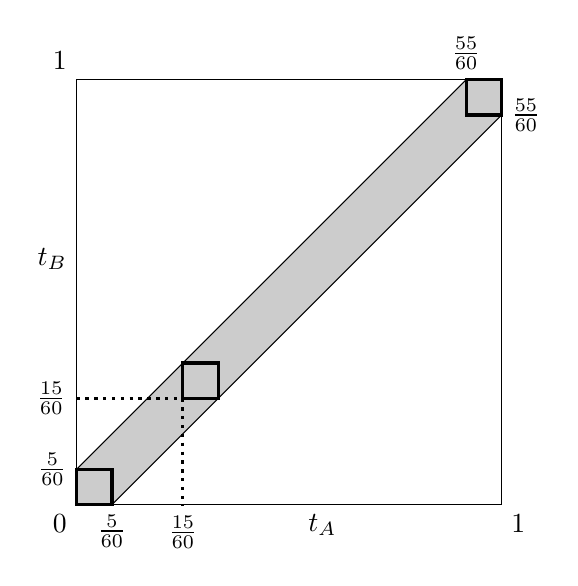
\begin{tikzpicture}[scale=.9]
\draw (0,0) -- node[below,xshift=12pt] {$t_A$} (6,0) -- (6,6) -- (0,6) -- node[left,yshift=12pt] {$t_B$} cycle;
\node[below left]  at (0,0) {$0$};
\node[below right] at (6,0) {$1$};
\node[above left]  at (0,6) {$1$};
\draw[fill=white!80!black]
  (0,0) -- 
  (.5,0) node[below] {$\frac{5}{60}$} -- 
  (6,5.5) node[right] {$\frac{55}{60}$} --
  (6,6) -- (5.5,6) node[above] {$\frac{55}{60}$} --
  (0,.5) node[left] {$\frac{5}{60}$} -- cycle;
\draw[very thick] (0,0) -- (.5,0) -- (.5,.5) -- (0,.5) -- cycle;
\draw[very thick] (1.5,1.5) -- ++(.5,0) -- ++(0,.5) --
  ++(-.5,0) -- cycle;
\draw[very thick] (5.5,5.5) -- ++(.5,0) -- ++(0,.5) --
  ++(-.5,0) -- cycle;
\draw[very thick,dotted] (0,1.5) node[left] {$\frac{15}{60}$} --
  (1.5,1.5) -- (1.5,0) node[below] {$\frac{15}{60}$};
\end{tikzpicture}
\end{center}
\caption{Times that ensure a meeting between $A$ and $B$}\label{f.duel}
\end{figure}
If $A$ arrives later, $B$ also has to arrive later by the same amount. For example, if $A$ arrives at $t_A=15$, $B$ must arrive between $t_B=15$ and $t_B=20$. Therefore, the meeting will take place during a square of time obtained by moving the square by $15$ along both axes from $(0,0)$ to $(15/60,15/60)$.

The probability of a meeting is the ratio of the area of the graph colored gray to the area of the large square. It is easier to compute the complement which is the ratio of the area of the two triangles to the area of the large square:
\begin{eqn}
P(A,B\;\textsf{meet}) &=& 1- P(A,B\;\textsf{don't meet})\\
&=&1- 2\cdot \left(\frac{1}{2}\cdot \frac{55}{60}\cdot \frac{55}{60}\right)=\frac{23}{144}\approx 0.1597\,.
\end{eqn}%

\textbf{Simulation}
\begin{verbatim}
Probability of meeting   = 0.1597
Proportion of meetings   = 0.1549
\end{verbatim}

%%%%%%%%%%%%%%%%%%%%%%%%%%%%%%%%%%%%%%%%%%%%%%%%%%%%%%%%%%%%%

\begin{prob}{Catching the cautious counterfeiter}

There are $n$ boxes each containing $n$ coins one of which is counterfeit. Draw one coin from each box and test it to determine whether it is counterfeit or genuine. What is the probability that all the coins that are drawn are real?

\que{1} Solve for $n=10$.

\que{2} Solve for $n=100$.

\que{3} Solve for arbitrary $n$.

\que{4} Develop a formula for limit of the probability as $n$ tends to infinity.
\end{prob}

\solution{}

The draws are independent so the probability is the product of the individual probabilities.

\ans{1}
\[
P(\textsf{all coins are genuine}) = \left(\frac{9}{10}\right)^{10}=0.3487\,.
\]


\ans{2}
\[
P(\textsf{all coins are genuine}) = \left(\frac{99}{100}\right)^{100}=0.3660\,.
\]

\ans{3}
\[
P(\textsf{all coins are genuine}) = \left(\frac{n-1}{n}\right)^{n}\,.
\]

\ans{4}
\begin{equation}\label{eq.reciprocal}
\lim_{n\rightarrow\infty}\left(1-\frac{1}{n}\right)^{n}=\frac{1}{e}\approx 0.3679\,.
\end{equation}

This limit can be proved using differential calculus. Compute the limit of the natural logarithm of the lefthand side of Equation~\ref{eq.reciprocal}:
\[
\lim_{n\rightarrow\infty}\ln \left(1-\frac{1}{n}\right)^{n}=
  \lim_{n\rightarrow\infty}n\ln \left(1-\frac{1}{n}\right)=
  \lim_{n\rightarrow\infty} \disfrac{\ln\left(1-\frac{1}{n}\right)}{1/n}\,.
\]
Taking the limit gives $(ln \;1)/0=0/0$ but by l'H\^{o}pital's rule we can replace expression by the quotient of the derivatives where we recall that $(\ln x)'=x'(1/x)$:
\begin{eqn}
\lim_{n\rightarrow\infty}\ln \left(1-\frac{1}{n}\right)^{n}&=&\lim_{n\rightarrow\infty}\frac{(-(-n^{-2}))\left(1-\frac{1}{n}\right)^{-1}}{-n^{-2}}=\lim_{n\rightarrow\infty}-\disfrac{1}{\left(1-\frac{1}{n}\right)}=-1\\
\lim_{n\rightarrow\infty}\left(1-\frac{1}{n}\right)^{n}&=&e^{-1}\,.
\end{eqn}%

\textbf{Simulation}
\begin{verbatim}
For  10 boxes:
Probability of all real = 0.3487
Proportion all real     = 0.3480
For 100 boxes:
Probability of all real = 0.3660
Proportion all real     = 0.3730
For 200 boxes:
Probability of all real = 0.3670
Proportion all real     = 0.3690
\end{verbatim}

%%%%%%%%%%%%%%%%%%%%%%%%%%%%%%%%%%%%%%%%%%%%%%%%%%%%%%%%%%%%%

\begin{prob}{Catching the greedy counterfeiter}
There are $n$ boxes each containing $n$ coins $m$ of which are counterfeit. Draw one coin from each box and test it to determine whether it is counterfeit or genuine. What is the probability $P(n,m,r)$ that $r$ of the coins that are drawn are counterfeit?

\que{1} Develop a formula for $P(n,m,r)$.

\que{2} Compute $P(20,10,2), P(20,10,8), P(20,5,2), P(20,5,4)$.
\end{prob}

\solution{}

\ans{1}
There are ${n\choose r}$ choices of boxes from which the counterfeit coins can be drawn. From the binomial distribution:
\[
P(n,m,r) = {n \choose r} \left(\frac{m}{n}\right)^r \left(\frac{n-m}{n}\right)^{n-r}\,.
\]

\ans{2}
\begin{eqn}
P(20,10,2) &=& \dischoose{20}{2} \left(\frac{10}{20}\right)^2 \left(\frac{10}{20}\right)^{18}\approx 0.0002\\
P(20,10,8) &=& \dischoose{20}{8} \left(\frac{10}{20}\right)^{8} \left(\frac{10}{20}\right)^{12}\approx 0.1201\\
P(20,5,2)&=&\dischoose{20}{2} \left(\frac{5}{20}\right)^2 \left(\frac{15}{20}\right)^{18}\approx 0.0669\\
P(20,5,4)&=&\dischoose{20}{4} \left(\frac{5}{20}\right)^{4} \left(\frac{15}{20}\right)^{16}\approx 0.1897\,.
\end{eqn}%

\textbf{Simulation}
\begin{verbatim}
For 10 bad coins,  2 draws:
Probability of counterfeit  = 0.0002
Proportion counterfeit      = 0.0002
For 10 bad coins,  8 draws:
Probability of counterfeit  = 0.1201
Proportion counterfeit      = 0.1181
For  5 bad coins,  2 draws:
Probability of counterfeit  = 0.0669
Proportion counterfeit      = 0.0688
For  5 bad coins,  4 draws:
Probability of counterfeit  = 0.1897
Proportion counterfeit      = 0.1905
\end{verbatim}

Using the limit from Problem~27, Mosteller shows that for $m,r$ given, as $n$ tends to infinity:
\begin{equation}\label{eq.bin-limit}
\lim_{n\rightarrow \infty}P(n,m,r) = \frac{e^{-m}m^r}{r!}\,.
\end{equation}
Here is a comparison of the probabilities for $m=10, r=8$ for increasing values of $n$:

\begin{verbatim}
Limit = 0.11259903, binomial = 0.11482303, n = 100
Limit = 0.11259903, binomial = 0.11282407, n = 1000
Limit = 0.11259903, binomial = 0.11262155, n = 10000
Limit = 0.11259903, binomial = 0.11259926, n = 1000000
\end{verbatim}

%%%%%%%%%%%%%%%%%%%%%%%%%%%%%%%%%%%%%%%%%%%%%%%%%%%%%%%%%%%%%

\begin{prob}{Moldy gelatin}

A rectangular plate is divided into $n$ squares with an average of $m$ microbes per square.

\que{1} Develop a formula for probability that there are exactly $r$ microbes in the $n$ squares.

\que{2} Compute the probability for $n=100, m=3, r=3$.

\textbf{Hint:} This problem is similar the Problem~28.

\end{prob}

\solution{}

\ans{1}
$p$, the probability that a single square contains a microbe (ignoring the possibility that a microbe is partially contained within two or more squares), is $m/n$. Then $P(n,m,r)$, the probability that there are exactly $r$ microbes in the $n$ squares, is given by the binomial distribution:
\[
P(n,m,r) = {n \choose r} \left(\frac{m}{n}\right)^r \left(\frac{n-m}{n}\right)^{n-r}\,.
\]

\ans{2} 
\[
P(10,3,3) = {100 \choose 3} \left(\frac{3}{100}\right)^3 \left(\frac{97}{100}\right)^{97}\approx 0.2275\,.
\]
\textbf{Simulation}
The simulations were run for $m=r=3$ and $m=r=5$.
\begin{verbatim}
For  20 squares:
Probability of exactly  3 microbes  = 0.2428
Proportion of exactly   3 microbes  = 0.2436
Probability of exactly  5 microbes  = 0.2023
Proportion of exactly   5 microbes  = 0.1954
For 100 squares:
Probability of exactly  3 microbes  = 0.2275
Proportion of exactly   3 microbes  = 0.2247
Probability of exactly  5 microbes  = 0.1800
Proportion of exactly   5 microbes  = 0.1851
\end{verbatim}

Equation~\ref{eq.bin-limit} also applies here to compute the limit as $n$ tends to infinity:
\begin{eqnarray*}
\lim_{n\rightarrow \infty}P(n,m,r) &=& \frac{e^{-m}m^r}{r!}\\
\lim_{n\rightarrow \infty} P(n,3,3) &=& \frac{e^{-3}\cdot 3^3}{3!}\approx 0.2240\\
\lim_{n\rightarrow \infty} P(n,5,5) &=& \frac{e^{-5}\cdot 5^5}{5!}\approx 0.1755\,.
\end{eqnarray*}

%%%%%%%%%%%%%%%%%%%%%%%%%%%%%%%%%%%%%%%%%%%%%%%%%%%%%%%%%%%%%

\refstepcounter{problem} % 30. Evening the sales

%%%%%%%%%%%%%%%%%%%%%%%%%%%%%%%%%%%%%%%%%%%%%%%%%%%%%%%%%%%%%

\begin{prob}{Birthday pairings}

\que{1} For $n$ people what is the probability $P(n)$ that two or more have the same birthday?

\que{2} What is the smallest value of $n$ such that $P(n)>0.5$?

Assume that the distribution of birthdays is uniform in the range $[1,365]$.

\textbf{Hint:} Compute the probability that $n$ people have \emph{different} birthdays and take the complement.
\end{prob}

\solution{}

\que{1}
Select the $n$ people one-by-one and check if they have the same birthday as the previous ones selected. For the first person you have $365$ days, for the second person you have $364$ days to choose from and so on:
\[
1-P(n)=
  \overbrace{\disfrac{365}{365}\cdot\frac{364}{365}
  \cdot \;\cdots \; \cdot \frac{365-(n-2)}{365}
  \cdot\frac{365-(n-1)}{365}}^{n}
=\disfrac{365!/(365-n)!}{365^{n}}\,.
\]
\que{2}
Compute this value for various values of $n$ or use a computer to loop from $1$ to $365$ until you find the first $n$ such that $1-P(n)<0.5$. This turns out to be $23$:
\[
1-P(23)=\disfrac{365!}{365^{23}\cdot 342!}\approx 0.4927\,.
\]
Most people are surprised that $23$ is the smallest value of $n$.

A modern calculator can compute $1-P(23)$ but it is a worthwhile exercise to compute it with Stirling's approximation $\ln n! \approx n\ln n - n$:
\begin{eqnarray*}
\ln (1-P(n))&=&
  \ln\left(\disfrac{365!}{342!\cdot 365^{23}}\right)=\ln 365! - \ln 342! -23 \ln 365\\
&\approx& (365\ln 365 -365) - (342\ln 342 -342) - 23\,\ln 365 \\
&\approx&-0.7404\\
1-P(n)&\approx&e^{-0.7404}=0.4769\,.
\end{eqnarray*}
The reader is invited to compute the probability with the following better approximation:
\[
\ln n!  \approx n\ln n - n + \frac{1}{6}\left(8n^3+4n^2+n+\frac{1}{30}\right)+\frac{1}{2}\ln\pi\,.
\]
\textbf{Simulation}
\begin{verbatim}
For 21 people:
Expectation of no pairs = 0.5563
Average no pairs        = 0.5497
For 22 people:
Expectation of no pairs = 0.5243
Average no pairs        = 0.5237
For 23 people:
Expectation of no pairs = 0.4927
Average no pairs        = 0.4933
For 24 people:
Expectation of no pairs = 0.4617
Average no pairs        = 0.4576
For 25 people:
Expectation of no pairs = 0.4313
Average no pairs        = 0.4345
\end{verbatim}

%%%%%%%%%%%%%%%%%%%%%%%%%%%%%%%%%%%%%%%%%%%%%%%%%%%%%%%%%%%%%

\begin{prob}{Finding your birthmate}
Your \emph{birthmate} is a person with the same birthday as yours.

Why is finding a birthmate a different problem than finding a birthday pair?

\que{1} How many people do you have to ask until the probability $Q(n)$ of finding your birthmate becomes greater than $0.5$?

\que{2}
Solve the problem by using the approximation in Equation~\ref{eq.reciprocal} (page~\pageref{eq.reciprocal}).
\end{prob}

\solution{}

Many people could have the same birthday which is considered a success for find a birthday pair, but not for finding a birthmate unless that birthday is the same as yours.

\ans{1}
We find $1-Q(n)$ the smallest number of people for which the probability that none of them are birthmates is less than $0.5$. The probability that the first person you ask is not a birthmate is $364/365$, but that is also the probability that the second, third, \ldots, person is not a birthmate. The solution is the smallest $n$ such that:
\[
1-Q(n)=\left(\frac{364}{365}\right)^n<\frac{1}{2}\,.
\]
By searching or writing a computer program we find that $n=253$:
\[
\left(\frac{364}{365}\right)^{253} \approx 0.4995\,.
\]
\ans{2}
Equation~\ref{eq.reciprocal} is:
\[
\lim_{n\rightarrow\infty}\left(1-\frac{1}{n}\right)^{n}=\frac{1}{e}\,,
\]
which can be used to approximate the probability:
\begin{eqn}
1-Q(n)&\approx &
  \left(1-\disfrac{1}{365}\right)^n=\left[\left(\disfrac{364}{365}\right)^{365}\right]^{n/365}\\
&\approx& e^{-n/365}\\
1-Q(253)&\approx&e^{-253/365}\approx 0.5000\,.
\end{eqn}%
\textbf{Simulation}
\begin{verbatim}
For 251 people:
Probability of no match = 0.5023
Proportion no match     = 0.5120
For 252 people:
Probability of no match = 0.5009
Proportion no match     = 0.5055
For 253 people:
Probability of no match = 0.4995
Proportion no match     = 0.4984
For 254 people:
Probability of no match = 0.4982
Proportion no match     = 0.4987
For 255 people:
Probability of no match = 0.4968
Proportion no match     = 0.5078
\end{verbatim}


%%%%%%%%%%%%%%%%%%%%%%%%%%%%%%%%%%%%%%%%%%%%%%%%%%%%%%%%%%%%%

\begin{prob}{Relating the birthday pairings and the birthmate problems}
Let $P(r)$ be the probability of finding a birthday pair (Problem~$31$) and let $Q(n)$ be the probability that out of $n$ people at least one is your birthmate (Problem~$32$). Given $r$ for what $n$ does $P(r) \approx Q(n)$?
\end{prob}

\solution{1}

The solution is based on \cite{birthday}.

From the solution to Problem~$31$ we have:
\[
\renewcommand*{\arraystretch}{2.2}
\begin{array}{lcl}
1-P(r)&=&
\disfrac{365}{365}\cdot 
  \frac{365-1}{365}\cdot \frac{365-2}{365} \cdot\;
  \cdots \;\cdot \frac{365-(r-1)}{365}\\
&=&1\left(1-\disfrac{1}{365}\right)
  \left(1-\disfrac{2}{365}\right) \cdot\;
  \cdots \;\cdot \left(1-\disfrac{r-1}{365}\right)\\
%&\approx&1-\disfrac{1}{365} - \disfrac{2}{365} -
%  \cdots - \disfrac{r-1}{365}\\
&\approx &1-\disfrac{1+2+3+\cdots + (r-1)}{365}\\
&=&1-\disfrac{r(r-1)/2}{365}\,,
\end{array}
\]
where the approximation in the third equation results from deleting powers of $1/365$ greater than one because they are too small to significantly affect the result.

Using the same approximation, from the solution to Problem~$32$ we have:
\[
\renewcommand*{\arraystretch}{2.2}
\begin{array}{lcl}
1-Q(n)
&=&\overbrace{\left(1-\frac{1}{365}\right)
  \left(1-\frac{1}{365}\right)\cdots
  \left(1-\frac{1}{365}\right)}^{n}\\
&\approx& 1-\overbrace{\frac{1}{365}-\frac{1}{365}\cdots-
  \frac{1}{365}}^{n}\\
&\approx& 1-\disfrac{n}{365}\\
\end{array}
\]
Therefore $P(r)\approx Q(n)$ when:
\[
n=\frac{r(r-1)}{2}\,.
\]
For $r=23$, $n=(23\cdot 22)/2=253$.

\solution{2}

Mosteller gives the following intuitive solution:
\begin{quote}
In comparing the birthday and birthmate problems, one observes that for $r$ people in the birthday problem, there are $r(r-1)/2$ pairs or \emph{opportunities} for like birthdays; whereas, if $n$ people are questioned in the birthmate problem, there are only $n$ opportunities for me to find one or more birthmates \cite[p.~322]{birthday}.
\end{quote}
From this he concludes that $n\approx r(r-1)/2$.

This reasoning can be understood as follows: For the birthday problem choose an arbitrary date and ask if two people out of $r$ have \emph{that birthday}. There are:
\[
{r \choose 2}=\frac{r!}{2!(r-2)!} = \frac{r(r-1)}{2}
\]
ways of doing so. For the birthmate problem your own birthday is given. Any of the $n$ people can have the same birthday. By equating the two expressions we have the $n$ such that $P_{\textsf{\footnotesize pair}}(r) \approx P_{\textsf{\footnotesize mate}}(n)$.

\medskip

\textbf{Simulation}

You can run the simulations using the programs for Problems~31, 32 and check this result.

%%%%%%%%%%%%%%%%%%%%%%%%%%%%%%%%%%%%%%%%%%%%%%%%%%%%%%%%%%%%%

\begin{prob}{Birthday holidays\annotate{D}}
A factory is closed whenever one of its workers has a birthday. There are no other holidays.

\que{1} How many workers should be employed in order to maximize the number of work-days in one year?

\que{2} What is the expectation of the ratio of the maximum work-days to $365^2$, the number of possible work-days if each one of $365$ workers worked every day?

\textbf{Hint:} Prove that there must be a maximum by considering extreme cases, then develop a formula for the expectation of the number of work-days for a single day.
\end{prob}

\solution{}

\ans{1}
At one extreme if there is only one worker there are $364$ work-days. If there are two workers there are $363+363=726$ workers days (ignoring the very small possibility that both workers have the same birthday). At the other extreme if there are one million workers the number of work-days will almost certainly be zero. Since the number of work-days rises initially and then returns to zero, there must be a maximum in between the extremes.

To simplify notation denote the number of days in a year by $N$ and the number of workers by $n$.

Let $p$ be the probability that a given day is a work-day, which is the probability that each worker has a birthday on some other day:
\[
p=\overbrace{\disfrac{N-1}{N} \cdot \;\cdots\;\cdot \disfrac{N-1}{N}}^n = \left(1-\disfrac{1}{N}\right)^n\,.
\]
On a work-day all workers work and on a holiday none do, so:
\[
E(\textsf{work-days for a given day}) = n \cdot p^n + 0\cdot (1-p^n) = np^n\,.
\]
All the days in the year have this same expectation so multiply by $N$ to get the expectation for a year:
\begin{equation}\label{eq.holidays}
E(\textsf{work-days for a year}) = Nnp^n\,.
\end{equation}

To find the maximum we take the derivative of Equation~\ref{eq.holidays} with respect to $n$ and use $(p^n)'=p^n\ln p$ which can be proved using the chain rule:
\[
(p^n)' = ((e^{\ln p})^n)' =
(e^{n\ln p})' =
(e^{n\ln p})' (n\ln p)'=
e^{n\ln p} \ln p=
(e^{\ln p})^n \ln p = p^n\ln p\,.
\]
The derivative of Equation~\ref{eq.holidays} is therefore:
\[
(Nnp^n)'= N (p^n + n (p^n)') = N (p^n + np^n\ln p)\,,
\]
which is $0$ when:
\[
n=-\disfrac{1}{\ln p}\,.
\]
For $N=365$ this gives $n=364.5$. Since $n$ is a positive integer the maximum is achieved at $n=364$ or $n=365$ which give the same expectation of the number of work-days:
\begin{eqn}
E(\textsf{work-days for a year}) &=&Nnp^n\\
&=&365\cdot 364 \cdot \left(\disfrac{364}{365}\right)^{364}\\
&=&365\cdot 364  \cdot \disfrac{365}{365}\left(\disfrac{364}{365}\right)^{364}\\
&=&365\cdot 365  \cdot \left(\disfrac{364}{365}\right)^{365}\\
&\approx &48944\,.
\end{eqn}%

\ans{2} 
The expectation of the ratio is:
\[
E(\textsf{max work-days/possible work-days})=\disfrac{365\cdot 365  \cdot \left(\frac{364}{365}\right)^{365}}{365\cdot 365}=\left(\disfrac{364}{365}\right)^{365}\approx 0.3674\,.
\]
By Equation~\ref{eq.reciprocal}:
\[
\lim_{n\rightarrow\infty}E(\textsf{max work-days/possible work-days})=\lim_{N\rightarrow \infty} \left(1-\disfrac{1}{N}\right)= \disfrac{1}{e}\,.
\]

\textbf{Simulation}
\begin{verbatim}
For 100 people
Expectation work-days    = 27742
Average work days        = 27743
Ratio work-days / 365**2 = 0.2082
For 250 people
Expectation work-days    = 45958
Average work days        = 45939
Ratio work-days / 365**2 = 0.3450
For 364 people
Expectation work-days    = 48944
Average work days        = 48936
Ratio work-days / 365**2 = 0.3674
For 365 people
Expectation work-days    = 48944
Average work days        = 48917
Ratio work-days / 365**2 = 0.3674
\end{verbatim}

%%%%%%%%%%%%%%%%%%%%%%%%%%%%%%%%%%%%%%%%%%%%%%%%%%%%%%%%%%%%%

\begin{prob}{The cliff-hanger}
A particle is initially placed on the $x$-axis at position $1$. At any position on the $x$-axis moves right with probability $2/3$ and left with probability $1/3$ (Figure~\ref{f.ruin1}).

\que{1} What is the probability that the particle will eventually be at position $0$?

\que{2} If the probability of moving right is $p$ and the probability of moving left is $1-p$, what is the probability that the particle will eventually be at position $0$? Analyze the result for various values of $p$.

\textbf{Hint:} Use conditional probabilities after the first move.
\begin{figure}[tb]
\begin{center}
\begin{tikzpicture}[scale=1.5]
\draw (0,0) -- (6,0);
\draw[dashed] (6,0) -- (8,0) node[right] {$\infty$};
\foreach \x in {0,1,2,3,4,5,6} {
  \draw (\x,0) -- +(0,4pt);
  \node at (\x,-10pt) { $\x$ };
}
\draw[fill] (1,5mm) circle[radius=.5pt];
\draw[->] (1,5mm) -- node[above] {$1/3$} (0,5mm);
\draw[->] (1,5mm) -- node[above] {$2/3$} (2,5mm);

\foreach \x/\y in {2/10mm,3/15mm,4/20mm} {
  \draw[fill] (\x,\y) circle[radius=.5pt];
  \draw[->] (\x,\y) -- node[above] {$1/3$} (\x-1,\y);
  \draw[->] (\x,\y) -- node[above] {$2/3$} (\x+1,\y);
}
\end{tikzpicture}
\end{center}
\caption{Can the particle return to $0$ (axis is infinite to the right)?}\label{f.ruin1}
\end{figure}
\end{prob}

\solution{}

\ans{1,2}
Denote a move left by $L$ and a move right by $R$. The particle can reach $0$ directly by moving $L$ with probability $\frac{1}{3}$, or by moving $RLL$ with probability $\frac{2}{3}\cdot\frac{1}{3}\cdot\frac{1}{3}$, or by moving $RRLLL$ with probability $\left(\frac{2}{3}\right)^2\left(\frac{1}{3}\right)^3$, \ldots\ . This computations seems to be a straightforward geometric progression, but it ignores possibilities such as $RLRLL$ so a different approach is needed.

Denote by $P(i,j)$ the probability that the particle reaches $i$ from $j$. Compute the probability that the particle reaches $0$ from $1$ conditioned on the first step:
\begin{eqn}
P(0,1) &=& P(0,1|\textsf{first move left}) +P(0,1|\textsf{first move right})\\
&=& (1-p)\cdot 1 + pP(1,2)P(0,1)\,.
\end{eqn}%
But $P(1,2) = P(0,1)$ giving a quadratic equation in $P(0,1)$:
\begin{eqn}
P(0,1) &=& (1-p) + pP(0,1)^2\\
pP(0,1)^2 - P(0,1) + (1-p) &=&0\\
%P&=& \frac{1\pm\sqrt{1-4p(1-p)}}{2p}\\
P(0,1)&=&1,\; \textsf{or}\; (1-p)/p\,.
\end{eqn}%
If $p\leq 1/2$ then $(1-p)/p\geq 1$, so $P(0,1)=1$ is the only solution and it is certain that the particle will reach $0$.

If $p=1$ then $P(0,1)=0$: if the particle always moves to the right it cannot return to $0$.

Suppose $P(0,1)=1$ for $1/2<p < 1$, that is, $P(0,1)$ \emph{does not} depend on $p$. In Figure~\ref{f.ruin2} the dashed red line shows the value $P(0,1)=1$ as $p$ approaches $1$ and the red dot shows $P(1,0)=0$ when $p$ becomes $1$. Since $P(0,1)$ cannot suddenly ``jump'' from $1$ to $0$,  the only solution is $P(0,1)=(1-p)/p$ for $p> 1/2$.\footnote{Mosteller writes that this follows by continuity but does not give a proof.}

\begin{figure}[tb]
\begin{center}
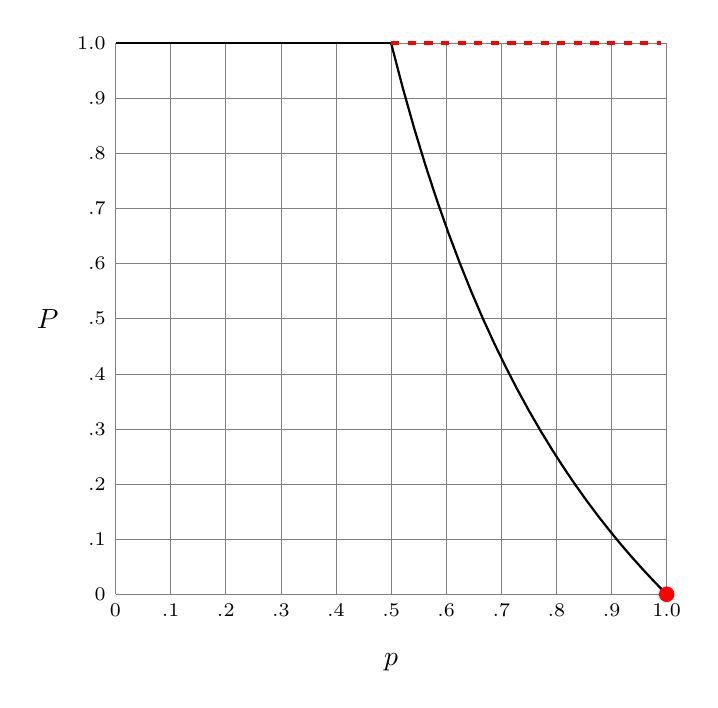
\begin{tikzpicture}[scale=7]
\draw[help lines,step=.1] (0,0) grid (1,1);
\foreach \x in {0,.1,.2,.3,.4,.5,.6,.7,.8,.9,1.0}
  \node[below] at (\x,0) {$\scriptstyle \x$};
\foreach \y in {0,.1,.2,.3,.4,.5,.6,.7,.8,.9,1.0}
  \node[left] at (0,\y) {$\scriptstyle \y$};
\draw[domain=0:.5,thick] plot (\x,1);
\draw[domain=.5:1,thick] plot (\x,{(1-\x)/\x});
\node at (.5,-3.5pt) {$p$};
\node at (-3.5pt,.5) {$P$};
\draw[ultra thick,red,dashed] (.5,1) -- +(.49,0);
\fill[red] (1,0) circle[radius=.4pt];
\end{tikzpicture}
\end{center}
\caption{Graph of $P=\min(p/(1-p),1)$ for $p\in [0,1]$}\label{f.ruin2}
\end{figure}
For $p=2/3, P$p> 1/2$=1/2$ and for $p=1/2, P$p> 1/2$=1$. This is surprising because one would not expect that the particle always returns to $0$ if the direction of the moves were determined by flipping a fair coin! You have to have a very unfair coin (probability of heads is $2/3$) to even the chances of returning to $0$.

\textbf{Simulation}
\begin{verbatim}
For probability = 0.2500:
Probability of reaching 0 = 1.0000
Proportion reaching 0     = 1.0000
For probability = 0.5000:
Probability of reaching 0 = 1.0000
Proportion reaching 0     = 0.9612
For probability = 0.6667:
Probability of reaching 0 = 0.5000
Proportion reaching 0     = 0.5043
For probability = 0.7500:
Probability of reaching 0 = 0.3333
Proportion reaching 0     = 0.3316
For probability = 0.8000:
Probability of reaching 0 = 0.2500
Proportion reaching 0     = 0.2502
\end{verbatim}

%%%%%%%%%%%%%%%%%%%%%%%%%%%%%%%%%%%%%%%%%%%%%%%%%%%%%%%%%%%%%

\begin{prob}{Gambler's ruin\annotate{D}}
A particle is initially placed on the $x$-axis at position $m\geq 1$. At any position on the $x$-axis moves right with probability $p>1/2$ and left with probability $1-p$.

\que{1} What is the probability that the particle will eventually be at position $0$?

\que{2} Let $n>m$. If the particle reaches position $0$ or position $n$ its stops moving (Figure~\ref{f.ruin3}). What is the probability that the particle will eventually be at position $0$? What is the probability that the particle will eventually be at position $n$?
\begin{figure}[tb]
\begin{center}
\begin{tikzpicture}[scale=1.5]
\draw (0,0) -- (6,0);
\foreach \x in {0,1,2,3,4,5,6} {
  \draw (\x,0) -- +(0,4pt);
  \node at (\x,-10pt) { $\x$ };
}
\node at (2,-20pt) {$m$};
\node at (6,-20pt) {$n$};
\draw[fill] (2,5mm) circle[radius=.5pt];
\draw[->] (2,5mm) -- node[above] {$1/3$} (1,5mm);
\draw[->] (2,5mm) -- node[above] {$2/3$} (3,5mm);
\end{tikzpicture}
\end{center}
\caption{What is the probability that the particle reaches $0$ or $n$?}\label{f.ruin3}
\end{figure}

\textbf{Note:} Problem~35 is represents a gambler with a finite amount of money playing against a casino with unlimited money. The problem asks for the probabiliy that the gambler loses all his money. Problem~36(2) represents one gambler who starts with $m$ playing against a second gambler who starts with $n-m$. The problem asks for the probabilities that \emph{one} of the gamblers loses all his money to the other one.
\end{prob}

\solution{}

The solution is based on \cite[Chapter~3, Example~4m]{ross}.

Denote by $P(i,j)$ the probability of reaching $i$ from $j$

\ans{1} The solution to Problem~35 showed that for $p>1/2$ (here it is given), if a particle is at position $1$ the probability of reaching position $0$ is $r=(1-p)/p$. This probability does not depend on the absolute position of the particle, that is:
\[
P(i,j) = P(i+k,k+1) = P(i-k,j-k)\,,
\]
therefore:
\begin{equation}
P(0,m)=P(m-1,m)P(m-2,m-1)\cdots P(1,2)P(0,1)=r^m\,.
\end{equation}

\ans{2} Abbreviate $P(n,i)$ by $P_i$ and compute $P_i$:
\begin{eqn}
P_i &=& pP_{i+1} + (1-p)P_{i-1}\\
%pP_{i+1}&=&1\cdot P_i - (1-p)P_{i-1}\\
pP_{i+1}&=&(p+(1-p))P_i - (1-p)P_{i-1}\\
p(P_{i+1}-P_i)&=&(1-p)(P_i-P_{i-1})\\
P_{i+1}-P_i&=&r(P_i-P_{i-1})\,.
\end{eqn}%
$P_0=0$ since if the particle is at $0$ it does not move. Therefore:
\begin{eqn}
P_2 - P_1 &=& r(P_1 - P_0) = rP_1\\
P_3 - P_2 &=& r(P_2 - P_1) = r^2P_1\\
\cdots &=&\cdots\\
P_i - P_{i-1} &=& r(P_{i-1} - P_{i-2}) = r^{i-1}P_1\,.
\end{eqn}%
Most of the terms on the lefthand sides cancel when we add the equations:
\begin{eqnlabels}
\nonumber{}P_i - P_1 &=& P_1\sum_{j=2}^{i}r^{j-1}\\
\nonumber{}&=& P_1 + P_1\sum_{j=2}^{i}r^{j-1} - P_1 \\
\label{eq.ruin0}P_i&=& P_1\sum_{j=0}^{i-1}r^j =P_1\left(\frac{1-r^i}{1-r}\right)\,.
\end{eqnlabels}
If the particle is at $n$ then it is already at $n$ so $P_n=1$:
\begin{eqnlabels}
\nonumber{}1 &=& P_1\left(\frac{1-r^n}{1-r}\right)\\
\label{eq.ruin00}P_1 &=& \left(\frac{1-r}{1-r^n}\right)\,.
\end{eqnlabels}
From Equations~\ref{eq.ruin0}, \ref{eq.ruin00}:
\begin{equation}
\label{eq.ruin1}P(n,i) = \left(\frac{1-r^{i}}{1-r^n}\right)\,.
\end{equation}
Using a symmetrical argument exchanging $p$ and $1-p$:
\begin{equation}
\label{eq.ruin2}P(0,i) = \left(\frac{1-(1/r)^{n-i}}{1-(1/r)^{n}}\right)\,.
\end{equation}
We leave it to the reader to show that the sum of Equations~\ref{eq.ruin1},~\ref{eq.ruin2} is $1$ meaning that one of the players will certainly win and one will lose. For $m=1, n=3, p=2/3$, r=1/2:
\begin{eqn}
P(0,1) &=& \left(\frac{1-\left(\frac{1}{2}\right)^{1}}{1-\left(\frac{1}{2}\right)^{3}}\right)=\frac{4}{7}\\
P(3,1) &=& \left(\frac{1-2^{2}}{1-2^{3}}\right)=\frac{3}{7}\,.
\end{eqn}%

\textbf{Simulation}
\begin{verbatim}
For probability = 0.6667:
Probability of reaching (0,10) from 1 = (0.4995,0.5005)
Proportion reaching     (0,10) from 1 = (0.5056,0.4944)
Probability of reaching (0,10) from 4 = (0.0616,0.9384)
Proportion reaching     (0,10) from 4 = (0.0643,0.9357)
Probability of reaching (0,10) from 6 = (0.0147,0.9853)
Proportion reaching     (0,10) from 6 = (0.0123,0.9877)
\end{verbatim}

\begin{verbatim}
For probability = 0.7500:
Probability of reaching (0,10) from 1 = (0.3333,0.6667)
Proportion reaching     (0,10) from 1 = (0.3395,0.6605)
Probability of reaching (0,10) from 4 = (0.0123,0.9877)
Proportion reaching     (0,10) from 4 = (0.0115,0.9885)
Probability of reaching (0,10) from 6 = (0.0014,0.9986)
Proportion reaching     (0,10) from 6 = (0.0015,0.9985)
\end{verbatim}
The greater the amount of money that the left player has and the greater his probability of winning each bet, the higher his probability of winning.

\textbf{Plot of steps}

This plot was generated by the Python library \texttt{matplotlib}; the source code appears in the file \texttt{36-gamblers-ruin-plot.py}.
\begin{center}
% This file was created with tikzplotlib v0.10.1.
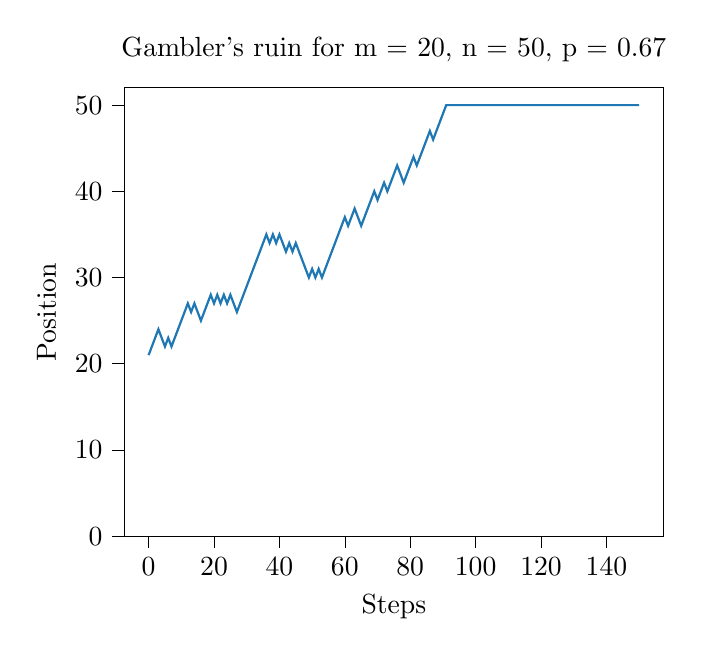
\begin{tikzpicture}

\definecolor{darkgray176}{RGB}{176,176,176}
\definecolor{steelblue31119180}{RGB}{31,119,180}

\begin{axis}[
tick align=outside,
tick pos=left,
title={Gambler's ruin for m = 20, n = 50, p = 0.67},
x grid style={darkgray176},
xlabel={Steps},
xmin=-7.5, xmax=157.5,
xtick style={color=black},
y grid style={darkgray176},
ylabel={Position},
ymin=0, ymax=52,
ytick style={color=black}
]
\addplot [thick, steelblue31119180]
table {%
0 21
1 22
2 23
3 24
4 23
5 22
6 23
7 22
8 23
9 24
10 25
11 26
12 27
13 26
14 27
15 26
16 25
17 26
18 27
19 28
20 27
21 28
22 27
23 28
24 27
25 28
26 27
27 26
28 27
29 28
30 29
31 30
32 31
33 32
34 33
35 34
36 35
37 34
38 35
39 34
40 35
41 34
42 33
43 34
44 33
45 34
46 33
47 32
48 31
49 30
50 31
51 30
52 31
53 30
54 31
55 32
56 33
57 34
58 35
59 36
60 37
61 36
62 37
63 38
64 37
65 36
66 37
67 38
68 39
69 40
70 39
71 40
72 41
73 40
74 41
75 42
76 43
77 42
78 41
79 42
80 43
81 44
82 43
83 44
84 45
85 46
86 47
87 46
88 47
89 48
90 49
91 50
92 50
93 50
94 50
95 50
96 50
97 50
98 50
99 50
100 50
101 50
102 50
103 50
104 50
105 50
106 50
107 50
108 50
109 50
110 50
111 50
112 50
113 50
114 50
115 50
116 50
117 50
118 50
119 50
120 50
121 50
122 50
123 50
124 50
125 50
126 50
127 50
128 50
129 50
130 50
131 50
132 50
133 50
134 50
135 50
136 50
137 50
138 50
139 50
140 50
141 50
142 50
143 50
144 50
145 50
146 50
147 50
148 50
149 50
150 50
};
\end{axis}

\end{tikzpicture}

\end{center}

%%%%%%%%%%%%%%%%%%%%%%%%%%%%%%%%%%%%%%%%%%%%%%%%%%%%%%%%%%%%%


\begin{prob}{Bold play vs. cautious play}
In roulette you can bet that the ball will fall into a pocket with an even number. The probability is $18/38$ since there are $18$ even numbers, $18$ odd numbers and $2$ green numbers. Which of the following strategies is better?
\begin{enumerate}
\item Bold play: bet $20$ in one round.
\item Cautious play: bet $1$ per round until you win or lose $20$.
\end{enumerate}
\textbf{Hint:} Use the results of Problem~36.
\end{prob}

\solution{}

The probability of winning with bold play is $18/38\approx 0.4737$.

Cautious play is the gambler's ruin problem (Problem~36): you start with $20$ and play until you reach $40$ (have won $20$) or until you reach $20$ (have lost it all). The probability of winning with cautious play is therefore given by Equation~\ref{eq.ruin1} with $p=18/38$ and $1-p=20/38$ so that $r=20/18$:
\[
P(40,20) =
\frac{1-(20/18)^{20}}{1-(20/18)^{40}}\approx 0.1084\,.
\]
Bold play is preferable to cautious play.

Mosteller writes that the intuitive explanation for this result is that betting in more rounds exposes the player to the probability of $2/38$ that the casino wins when the ball falls on a green number.

\newpage

\textbf{Simulation}
\begin{verbatim}
Probability of bold wins     = 0.4737
Proportion bold wins         = 0.4677
Probability of cautious wins = 0.1084
Proportion cautious wins     = 0.1094
\end{verbatim}

%%%%%%%%%%%%%%%%%%%%%%%%%%%%%%%%%%%%%%%%%%%%%%%%%%%%%%%%%%%%%

\refstepcounter{problem}

%%%%%%%%%%%%%%%%%%%%%%%%%%%%%%%%%%%%%%%%%%%%%%%%%%%%%%%%%%%%%

\begin{prob}{The clumsy chemist}

You have a large number of glass rods of length $1$ with one end colored red (hatched) and the other colored blue (dotted). When you drop them on the floor they each break into three pieces with a uniform distribution of the length of the pieces (\ref{f.rod1}). What is the expectation of the length of the piece whose end is colored blue?

\textbf{Hint:}
Instead of straight rods suppose that you are given (unmarked) glass rings that also break into three pieces (\ref{f.rod2}).
\begin{figure}[tb]
\begin{center}
\begin{subfigure}{.4\textwidth}
\begin{tikzpicture}
\draw (0,0) -- ++(6,0) -- ++(0,12pt) -- ++(-6,0) -- cycle;
\fill[pattern=crosshatch,pattern color=red]
  (0,0) rectangle +(12pt,12pt);
\fill[pattern=crosshatch dots,pattern color=blue]
  (6,0) rectangle +(-12pt,12pt);
\draw[<->] (0,23pt) --
  node[fill=white] {$1$} ++(6,0);
\draw[decorate,decoration=saw] (1.8,35pt) -- +(0,-55pt);
\draw[decorate,decoration=saw] (4.5,35pt) -- +(0,-55pt);
\draw[<->] (0,-10pt) --
  node[fill=white] {$\scriptstyle l_1$} (1.8,-10pt);
\draw[<->] (1.8,-10pt) --
  node[fill=white] {$\scriptstyle l_2$} (4.5,-10pt);
\draw[<->] (4.5,-10pt) --
  node[fill=white] {$\scriptstyle l_3$} (6,-10pt);
\path (0,-1) rectangle +(2,-1.5);
\end{tikzpicture}
\caption{Breaking a rod into three pieces}\label{f.rod1}
\end{subfigure}
\hspace{3em}
\begin{subfigure}[b]{.4\textwidth}
\begin{tikzpicture}
\draw (0,0) circle[radius=2];
\draw (0,0) circle[radius=1.6];
\draw[decorate,decoration=saw] (30:1) -- +(30:1.5);
\draw[decorate,decoration=saw] (190:1) -- +(190:1.5);
\draw[decorate,decoration=saw] (-90:1) -- +(-90:1.5);
\node[rotate=-4,minimum width=11pt,minimum height=11pt,
      pattern=crosshatch,pattern color=red]
  at (-94:1.8) {};
\node[rotate=6,minimum width=11pt,minimum height=11pt,
      pattern=crosshatch dots, pattern color=blue]
  at (-82:1.8) {};
\end{tikzpicture}
\caption{Breaking a ring into three pieces}\label{f.rod2}
\end{subfigure}
\end{center}
\end{figure}
\end{prob}

\solution{1}

The rods are not symmetric because the end pieces are different from the center piece. However, the ring is symmetric so the distributions of all three pieces must be uniform with expectation $1/3$. By choosing and coloring one of breaks as shown in \ref{f.rod2}, the problem is now the same as that of the rods so the distributions remain the same, and therefore the expectation of the lengths of the pieces is also $1/3$.

\solution{2}

Here is an elegant solution from \cite{stack-rods}.

Assume that the rod represents the line segment $(0,1)$. The rod is broken in two places which are represented as two uniform independent random variables $X,Y\in (0,1)$. Let us compute the probability $P(|X-Y|>a)$.

Table~\ref{t.rods} shows points $(x,y)$, where $x,y \in \{0.0, 0.1, 0.2, \ldots, 0.9\}$ and the decimal point is omitted. The values that appear in the table are $|X-Y|$. For $a=0.6$ the entries in the upper left corner (denoted in bold) and the entries in the lower right corner (denoted in bold) are the outcomes for which $P(|X-Y|>a)$:
\[
G(a) = P(|X-Y|>a)=2\cdot \frac{1}{2}(1-a)(1-a)=(1-a)^2\,.
\]
We are interested in the complment:
\[
F(a)=1-G(a)=P(|X-Y|<a)=1-(1-a)^2=2a-a^2\,.
\]
This is the cumulative probability distribution (CPD) for the interval $(0,1)$. 
\begin{table}[bt]
\[
\begin{array}{c}
\quad\\\\\\
a\\\\
\quad\\
y\\
\quad\\\quad\\\quad\\\quad
\end{array}
\begin{array}{|c|cccccccccc|}
\multicolumn{11}{l}{\qquad \qquad \qquad a}\\
\hline
9& \mathbf{9} & \mathbf{8} & \mathbf{7} & \mathbf{6} & 5 & 4 & 3 & 2 & 1 & 0  \\
8& \mathbf{8} & \mathbf{7} & \mathbf{6} & 5 & 4 & 3 & 2 & 1 & 0 & 1  \\
7& \mathbf{7} & \mathbf{6} & 5 & 4 & 3 & 2 & 1 & 0 & 1 & 2  \\
6& \mathbf{6} & 5 & 4 & 3 & 2 & 1 & 0 & 1 & 2 & 3  \\
5& 5 & 4 & 3 & 2 & 1 & 0 & 1 & 2 & 3 & 4  \\
4& 4 & 3 & 2 & 1 & 0 & 1 & 2 & 3 & 4 & 5  \\
3& 3 & 2 & 1 & 0 & 1 & 2 & 3 & 4 & 5 & \mathbf{6}  \\
2& 2 & 1 & 0 & 1 & 2 & 3 & 4 & 5 & \mathbf{6} & \mathbf{7}  \\
1& 1 & 0 & 1 & 2 & 3 & 4 & 5 & \mathbf{6} & \mathbf{7} & \mathbf{8}  \\
0& 0 & 1 & 2 & 3 & 4 & 5 & \mathbf{6} & \mathbf{7} & \mathbf{8} & \mathbf{9}  \\
\hline
&0 & 1 & 2 & 3 & 4 & 5 & 6 & 7 & 8 & 9  \\
\hline
\multicolumn{11}{c}{\quad \quad x\quad\quad\quad a}
\end{array}
\begin{array}{c}
\\\\\\
a\\\\
\end{array}
\]
\caption{Distribution of breaks on $(0,1)\times (0,1)$}\label{t.rods}
\end{table}
The probability density function (PDF) can be obtained by differentiating the CDP:
\[
f(a)=P(|X-Y|=a)= \frac{d}{da}F(a) =
  \frac{d}{da}(2a-a^2)=2(1-a)\,.
\]
The expectation is the integral of the PDF multiplied by the value:
\[
E(|X-Y|)= \int_{0}^{1} a\cdot2(1-a)\, da=
  2\left.\left(\frac{a^2}{2}-\frac{a^3}{3}\right)\right|_0^1=\frac{1}{3}\,.
\]

\textbf{Simulation}
\begin{verbatim}
Expectation of length of right piece = 0.3333
Average length of right piece        = 0.3359
\end{verbatim}

%%%%%%%%%%%%%%%%%%%%%%%%%%%%%%%%%%%%%%%%%%%%%%%%%%%%%%%%%%%%%

\begin{prob}{The first ace}
Deal cards from the top of a well-shuffled deck of cards until an ace appears. What is the expectation of the number of cards that must be dealt?

\textbf{Hint:} Consider the deck of cards without the aces laid out in a row.
\end{prob}

\solution{}

The cards form a ``rod'' of length $48$ which is ``broken'' by the $4$ aces into $5$ ``pieces.'' From Problem~39 the expectation of the length of a ``piece'' is $48/5=9.6$.

\textbf{Simulation}
\begin{verbatim}
Expectation of first ace = 9.6000
Average first ace        = 9.5805
\end{verbatim}

%%%%%%%%%%%%%%%%%%%%%%%%%%%%%%%%%%%%%%%%%%%%%%%%%%%%%%%%%%%%%
